\documentclass[10pt,a4paper]{article}
\usepackage[utf8]{inputenc}

\usepackage{amsmath}
\usepackage{amsfonts}
\usepackage{amssymb}
\usepackage{tikz}

\parindent 0pt


\begin{document}
\tableofcontents

\section{Introduction}
\subsection{Multiplication}
This equation $\displaystyle{5 \times 3 = 15}$ means 5 groups of 3 is 15.\\
\subsubsection*{Examples}

\begin{enumerate}
	\item $2 + 2 + 2 + 2 + 2 + 2 = 6 \times 2 = 12$
	\item $4 \times 3 = 3 + 3 + 3 + 3 = 12$
	\item $3 \times 4 = 4 + 4 + 4 + 4 = 12$
\end{enumerate}

\subsubsection*{Exmaple with number line}
$4 \times 2 = 8$ is represented by the following number line.\\

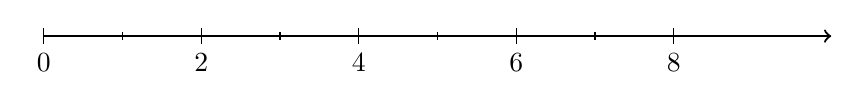
\begin{tikzpicture}
    % Draw the line
    \draw[thick, ->] (0,0) -- (10,0);

    % Draw ticks and labels
    \foreach \x in {0,2,4,6,8}
        \draw (\x,0.1) -- (\x,-0.1) node[below] {\x};

    % Draw an extra tick for the arrow (optional)
    % \draw (5,0.1) -- (5,-0.1) node[below] {5};
    
        % Add labels for every unit between -8 and 8
    \foreach \x in {0,1,3,5,7}
        \draw (\x,0.05) -- (\x,-0.05);
\end{tikzpicture}

\subsubsection{Commutative property of multiplication}

3 groups of 4 is equivalent with 4 groups of 3: $3 \times 4 = 4 \times 3 = 12$

\subsubsection{Distributive property of multiplication}
$4 \times 7 = 4 \times \left(5 + 2\right) = \left(4 \times 5\right) + \left(4 \times 2\right) = 28$\\\\
This techniques could be break down an complex problem into eaiser one.

\subsubsection{Associative property of multiplication}
$4 \times 5 \times 2 = \left(4 \times 5\right) \times 2 = 4 \times \left(5 \times 2\right) = 40$\\\\
The order of multiplication does not matter, but simplify the equation.\\
Such As:
$$5 \times 18 = 5 \times \left(2 \times 9\right) = \left(5 \times 2\right) \times 9 = 10 \times 9 = 90$$

\subsection{Division}





\end{document}